\section{Introduktion}
\begin{frame}
\frametitle{PsyLog platformen}
	\begin{itemize}
	\item Modulær platform til indsamling og analyse af data
	\item Gør det nemt at udvikle moduler som tilbyder ny funktionalitet
	\item Fokus på mentalt helbred
	\item Præsentation i dag vil omhandle udvikling af moduler dertil
	\end{itemize}
\end{frame}

\section{Mentalt helbred}
\begin{frame}
\frametitle{Indikatorer på mentalt helbred}
	\begin{itemize}
	\item Ændring i søvnvaner og aktivitetsniveau
	\item Fokus på søvn, da søvn er noget af det mest centrale ifølge flere personer
	\item Søvn kan svinge i begge retninger: For lidt eller for meget
	\item God indikator for unipolar eller bipolar depression
	\end{itemize}
\end{frame}

\section{Soevn}
\begin{frame}
\frametitle{Krav til søvnestimering}
	\begin{itemize}
	\item Undgå brugerintervention
	\item Brug i eget hjem
	\item Være præcis
	\end{itemize}
\end{frame}

\section{Forarbejde til søvnestimering}
\begin{frame}
\frametitle{Metoder}
	\begin{itemize}
	\item Kan vi benytte eksisterende metoder?
	\item Hvilke metoder er der?
	{\begin{itemize}
		\item Polysomnografi
		\item Toss'N'Turn
		\item Best Effort Sleep
		 \end{itemize}}
	\end{itemize}
\end{frame}

\begin{frame}
\frametitle{Polysomnografi}
\begin{figure}
	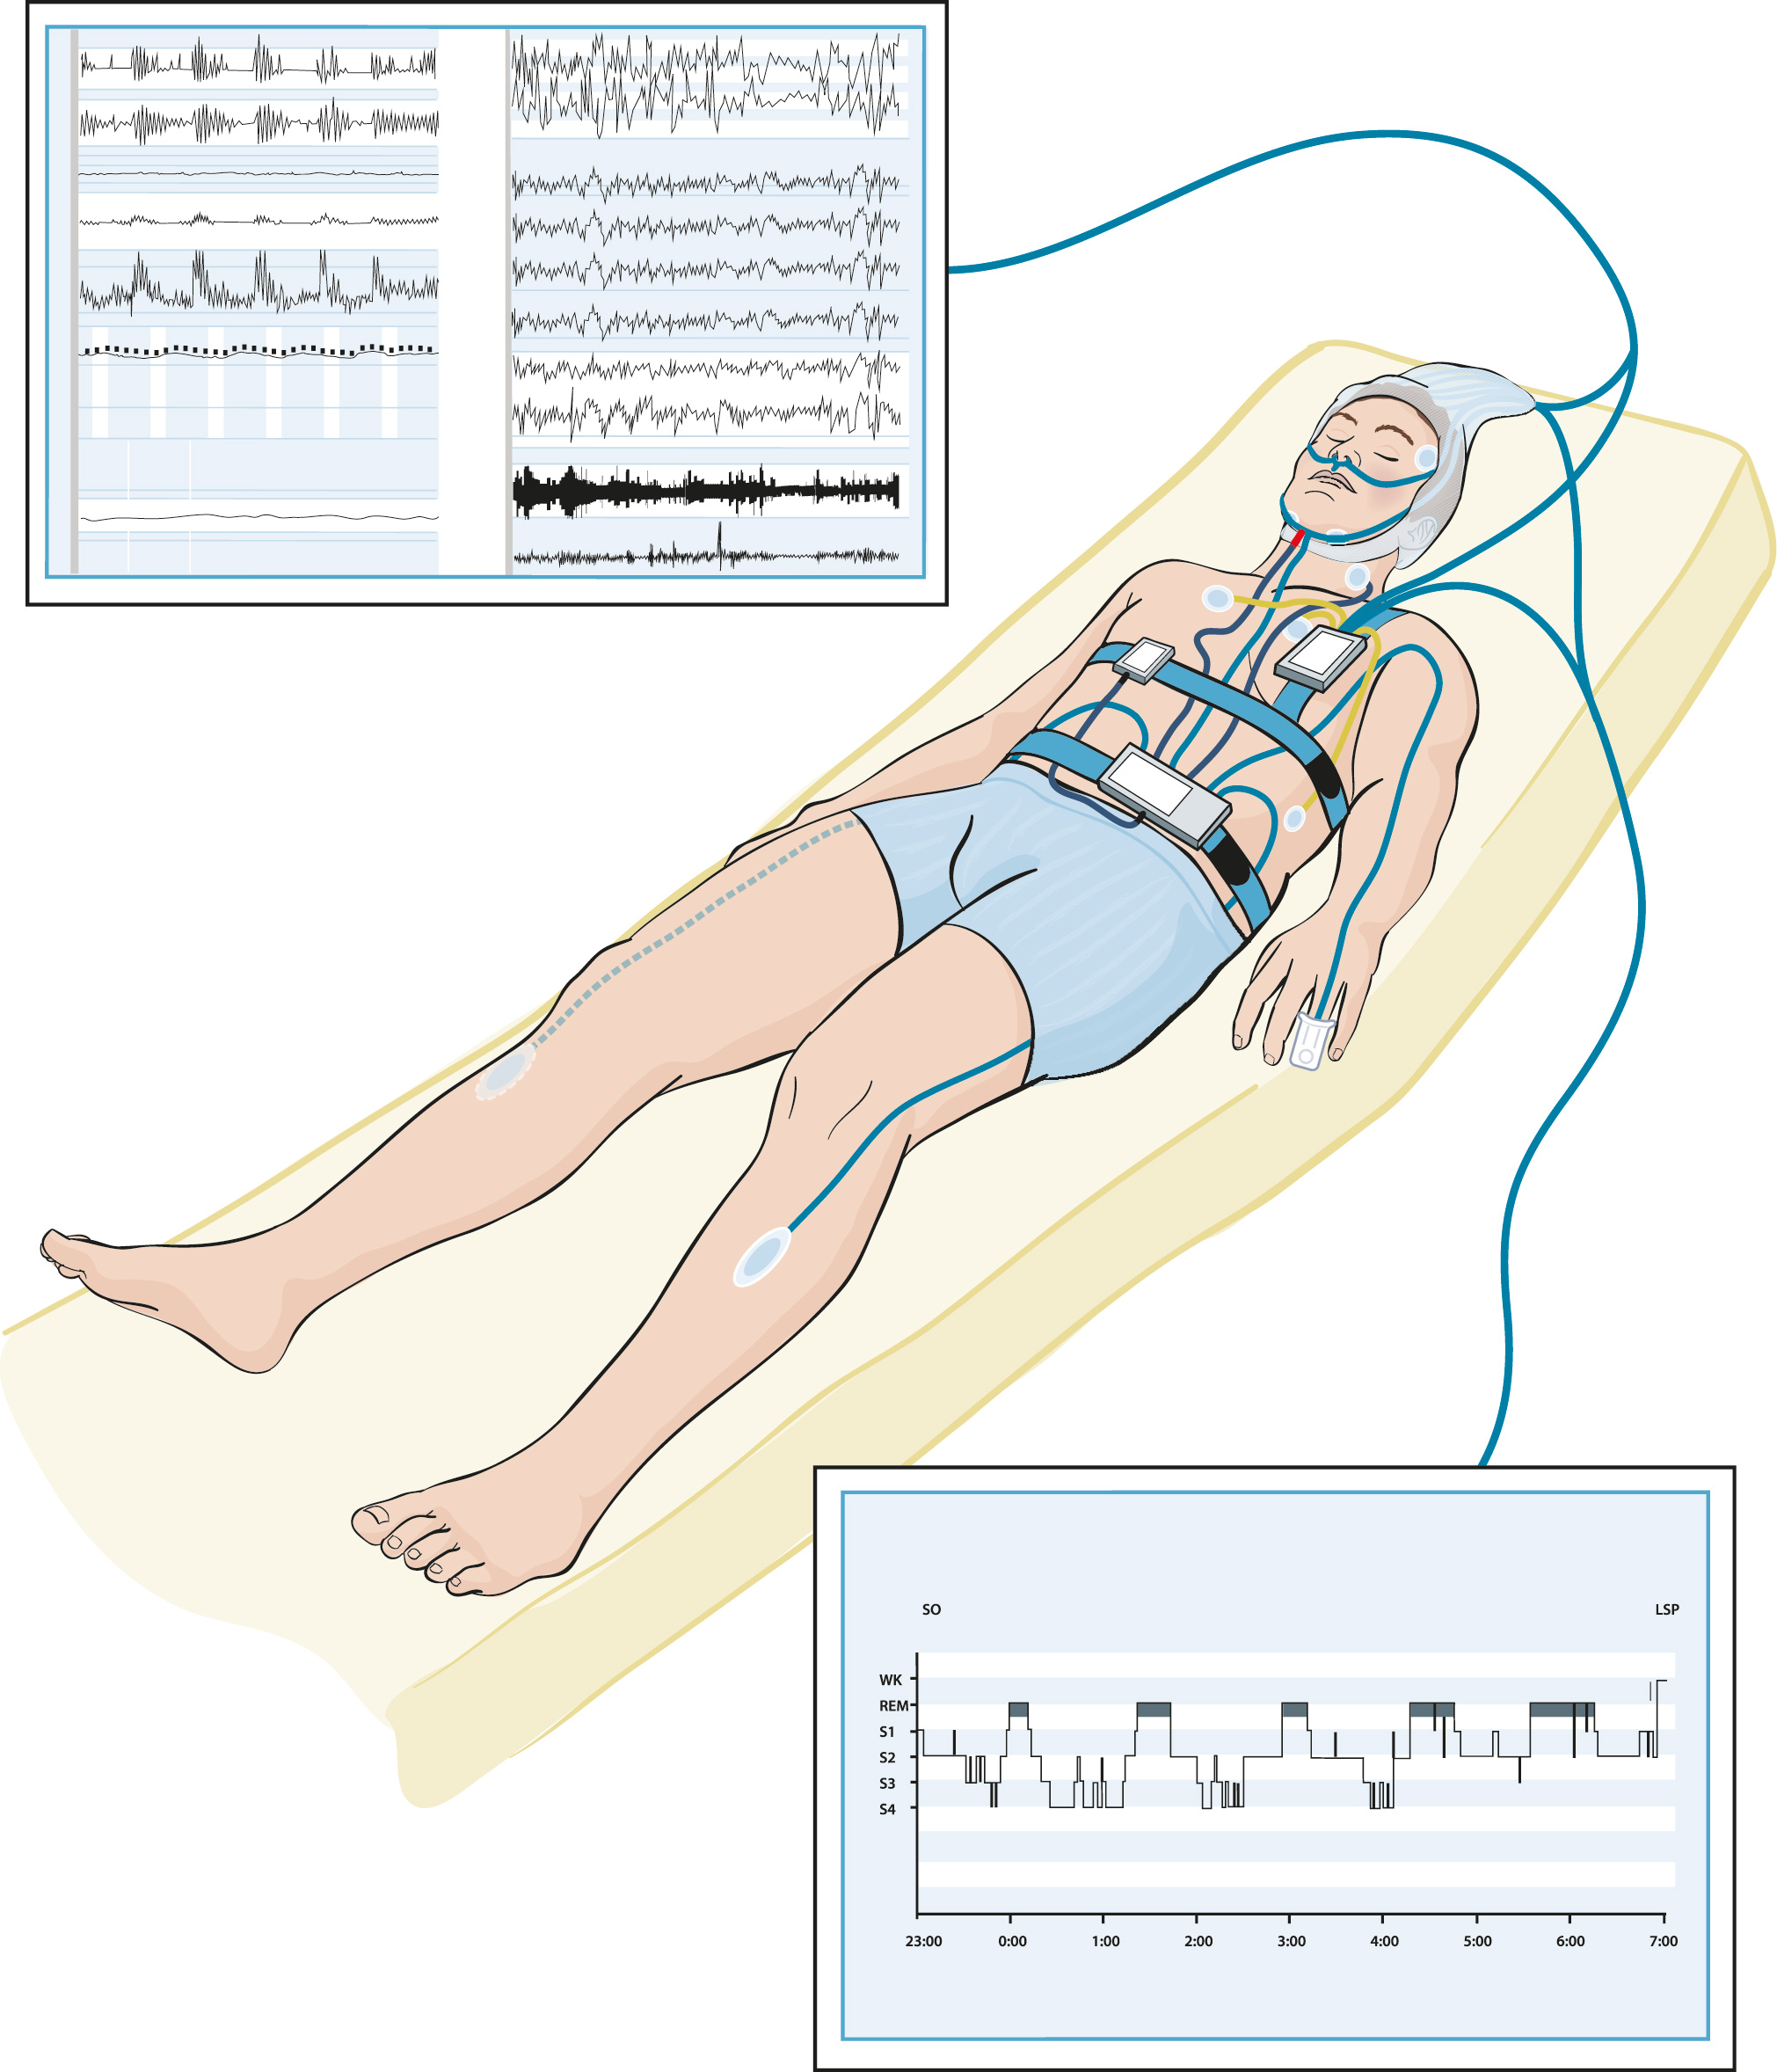
\includegraphics[scale=0.05]{polysomnografi}
\end{figure}

\begin{itemize}
	\item State of the art
	\item Kræver ekspert viden og specialudstyr og kan ikke bruges af en patient i eget hjem
\end{itemize}
\end{frame}

\begin{frame}
\frametitle{Toss'N'Turn}
\begin{itemize}
	\item 92\% nøjagtig søvnlængdeestimering
	\item Læringsperiode
\end{itemize}
\end{frame}

\begin{frame}
	\frametitle{Best Effort Sleep}
	\begin{itemize}
		\item 92\% nøjagtig søvnlængdeestimering
	\end{itemize}
\end{frame}

% Nu vil als så forsætte